% Sketch output, version 0.3 (build 7d, Wed Oct 26 10:57:35 2016)
% Output language: PGF/TikZ,LaTeX
\documentclass[letterpaper,12pt]{article}
\usepackage[x11names,rgb]{xcolor}
\usepackage{tikz}
\usetikzlibrary{snakes}
\usetikzlibrary{arrows}
\usetikzlibrary{shapes}
\usetikzlibrary{backgrounds}
\usepackage{amsmath}
\oddsidemargin 0in
\evensidemargin 0in
\topmargin 0in
\headheight 0in
\headsep 0in
\textheight 9in
\textwidth 6.5in
\begin{document}
\pagestyle{empty}
\vspace*{\fill}
\begin{center}
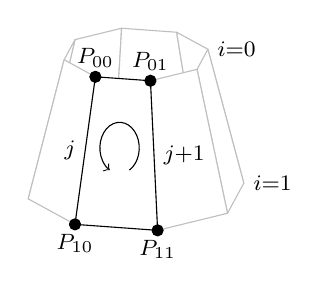
\begin{tikzpicture}[line join=round]
\tikzstyle{ann} = [fill=white,font=\footnotesize,inner sep=1pt]\filldraw[draw=lightgray,fill=white](-.775,1.922)--(-1.162,.283)--(-.274,.5)--(-.183,2.067)--cycle;
\filldraw[draw=lightgray,fill=white](-.183,2.067)--(-.274,.5)--(.775,.424)--(.516,2.016)--cycle;
\filldraw[draw=lightgray,fill=white](.516,2.016)--(.775,.424)--(1.369,.1)--(.913,1.8)--cycle;
\filldraw[draw=lightgray,fill=white](-.913,1.667)--(-1.369,-.1)--(-1.162,.283)--(-.775,1.922)--cycle;
\filldraw[draw=lightgray,fill=white](.913,1.8)--(1.369,.1)--(1.162,-.283)--(.775,1.545)--cycle;
\filldraw[draw=lightgray,fill=white](-.516,1.45)--(-.775,-.424)--(-1.369,-.1)--(-.913,1.667)--cycle;
\filldraw[draw=lightgray,fill=white](.775,1.545)--(1.162,-.283)--(.274,-.5)--(.183,1.4)--cycle;
\filldraw[fill=white](-.516,1.45)--(-.775,-.424)--(.274,-.5)--(.183,1.4)--cycle;
\filldraw(-.775,-.424) circle (2pt);
\filldraw(.274,-.5) circle (2pt);
\filldraw(-.516,1.45) circle (2pt);
\filldraw(.183,1.4) circle (2pt);
\fill[black,font=\footnotesize]
                (-.516,1.45) node [above] {$P_{00}$}
                (-.775,-.424) node [below] {$P_{10}$}
                (.183,1.4) node [above] {$P_{01}$}
                (.274,-.5) node [below] {$P_{11}$};\draw (-.209,.482)+(-60:.25) [yscale=1.3,->] arc(-60:240:.25);\path[font=\footnotesize] 
          (-.645,.513) node[left] {$j$}
          (.228,.45) node[right] {$j\hbox{$+$}1$};\path[font=\footnotesize]
          (.913,1.8) node[right] {$i\hbox{$=$}0$}
          (1.369,.1) node[right] {$i\hbox{$=$}1$};\end{tikzpicture}
\end{center}
\vspace*{\fill}
\end{document}
% End sketch output
